\section{\Large PROBLEM SET 9}

\subsection{Problem 1 - Start selecting and sizing your actuators using the basic dimensional formulas provided in class (Wertz, SMAD) based on your perturbation environment and attitude slew objectives. Provide rationale for choice.}

As shown in Section \ref{sec:pertTorques}, the total torque from aerodynamic drag, solar radiation, gravity, and magnetic disturbances are shown in Figure \ref{fig:all_torque} and again below in Figure \ref{fig:all_torque_hw9} for completeness.

\begin{figure}[H]
    \centering
    \captionsetup{ justification = centering }
    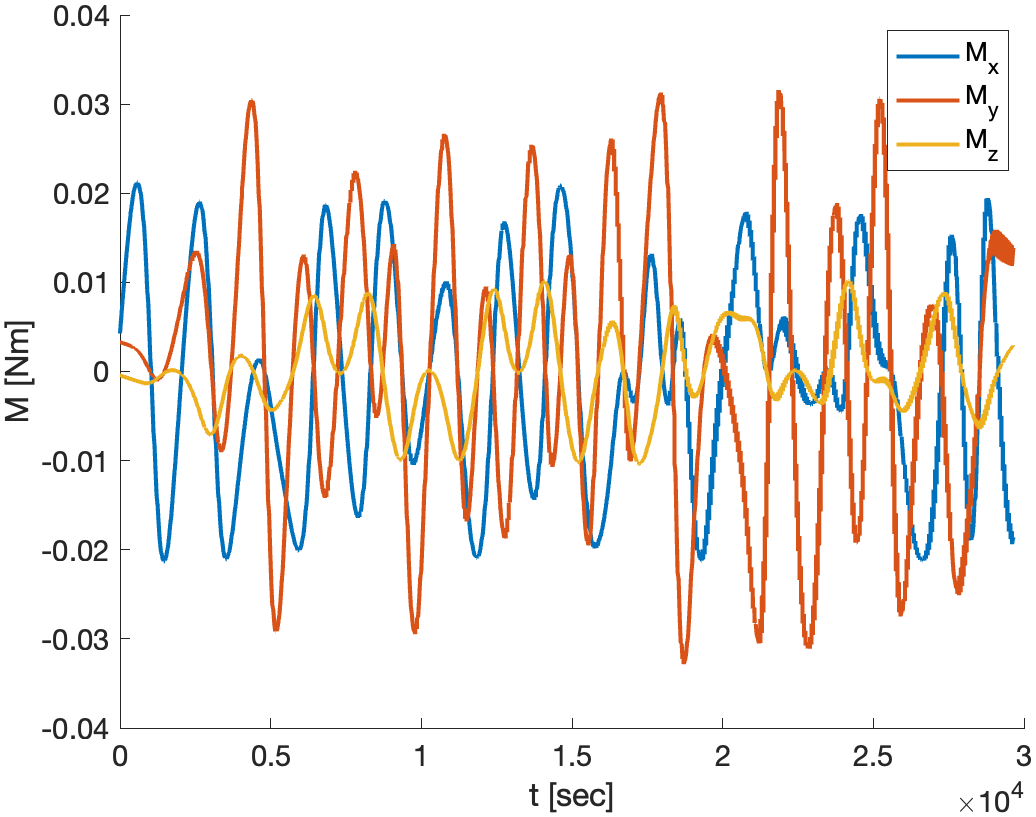
\includegraphics[width = 12cm]{Images/PS6/all_torque.png}
    \caption{Total Torque}
    \label{fig:all_torque_hw9}
\end{figure}

In this plot it can be seen that the maximum torque is about 0.035 Nm. Due to the criticality of the actuators to the mission, a safety factor of 2.5 was selected to ensure that the selected actuators would be well equipped to handle perturbations well outside of the expected range. Multiplying the safety factor by the maximum perturbation torque resulted in a required maximum torque of 0.0875 Nm. Due to the nature of the mission, it isn't required for the satellite to complete fast slew maneuvers to switch between different modes of operation. Because the satellite is in a sun-synchronous orbit, and the sensors will always be earth pointing, there isn't a need to quickly slew between the science mode of operation where the data collection is prioritized to the charging mode of operation where the solar arrays must be pointed towards the sun. Because of this, it is sufficient to size the actuators to handle the manuevers that are needed to correct for perturbations torques and not for fast slew maneuvers.

In order to ensure that the chosen actuators were able to produce the required maximum torque, available data sheets for momentum/reaction wheels and magnetorquers were analyzed. For reaction wheels, the Rocket Lab 12.0 Nms RW4 [Rad-Hard] and RW5 [Standard] were analyzed as well as the Bradford Aerospace High Torque Reaction Wheel for Satellites. Their maximum angular momentum and torque outputs are tabulated in Table \ref{table:rw}.

\begin{table}
\begin{tabular}{c|c|c}
    & Maximum Angular Momentum (Nms) & Maximum Torque (Nm) \\
    \hline 
    Bradford & 45 & 0.265 \\
    \hline 
    Rocket Lab & 12 & 0.2 \\
\end{tabular}
\caption{Reaction Wheel Data}
\label{table:rw}
\end{table}

It can also be noted that for the Bradford reaction wheel the torque rise/fall time was listed as 80 ms. Because of this short rise time, the initial angular momentum of the reaction wheel can be approximated as being anything between zero and the maximum value. For the magnetorquer, the maximum and nominal dipole moments were collected for the AAC Clyde Space MTQ800 magnetorquer and are tabulated in Table \ref{table:magnetorquer}.

\begin{table}
\begin{tabular}{c|c|c}
    & Maximum Dipole Moment (Am$^2$) & Nominal Dipole Moment (Am$^2$) \\
    \hline 
    AAC & 30 & 15 \\
\end{tabular}
\caption{Magnetorquer Data}
\label{table:magnetorquer}
\end{table}

While the exact torque output wasn't given in the specifications for the magnetorquer, it can be assumed that it is between 5e-4 and 5e-1 Nm for the given specifications. 

Due to the reaction wheels being large enough to handle the perturbation torques and the magnetorquers being better suited for fine tuning, we decided to use a combination of a set of reaction wheels and magnetorquers for the satellite.

\subsection{Problem 2 - Start modeling actuators in dedicated (Simulink) subsystems which are part of the spacecraft. These models take inputs from ground-truth simulation and provides output control torques to be directly fed into the Euler equations, including systematic and random errors. Plot output vs input of actuator model. Hint: for the rest of this problem set you should remove all sensing and actuation errors for verification purposes.}

For our actuators, we modelled a reaction wheel, momentum wheel, and a magnetorquer. For the reaction wheel and momentum wheel, we started with the Euler equation shown below.

\begin{equation}
    \Vec{\dot L}_t + \Vec{\omega} \times \Vec{L}_t = \Vec{M}
\end{equation}

Substituting in $\Vec{L}_t = \Vec{I} \Vec{\omega} + \Vec{A} \Vec{L}_w$ where $\Vec{A}$ is used to bring the angular momentum of the wheels into the principle axes into the above equation gives the full Euler equation.

\begin{equation}
    \Vec{I} \Vec{\dot \omega} + \Vec{\dot I} \Vec{\omega} + \Vec{A} \Vec{\dot L}_w + \Vec{\dot A} \Vec{L}_w + \Vec{\omega} \times \Vec{I} \Vec{\omega} + \Vec{\omega} \times \Vec{A} \Vec{L}_w = \Vec{M}
\end{equation}

For one reaction wheel and one momentum wheel, the equation can be simplified to the form shown below.

\begin{equation}
    \Vec{\dot L}_w = \Vec{A}^* \left( - \Vec{M}_c - \Vec{\omega} \times \Vec{A} \Vec{L}_w \right)
\end{equation}

From substituting in moment of inertias and angular velocities and linearizing, we obtain the following set of equations.

\begin{align}
    I_x (\Ddot{\alpha}_x - n \dot \alpha_y ) + (I_z - I_y) ( n \dot \alpha_y + n^2 \alpha_x ) + I_{wz}\Bar{\omega}_{wz} ( \dot \alpha_y + n \alpha_x) - I_{wy} \omega_{wy} n = 0
\end{align}

\begin{align*}
    I_x (\Ddot{\alpha}_y - n \dot \alpha_x ) + (I_z - I_y) ( n \dot \alpha_x - n^2 \alpha_y ) - I_{wz}&\Bar{\omega}_{wz} ( \dot \alpha_x + n \alpha_y) + I_{wy} \omega_{wy} - 3 n^2 (I_x - I_z) \alpha_y = 0 \\
    I_z \Ddot{\alpha}_z + I_{wz} \dot \omega_{wz} +& 3n^2\left( I_y - I_x \right) \alpha_z = 0 \\
    I_{wy} \dot \omega_{wy} = M_{cy} ;& I_{wz} \dot \omega_{wz} = M_{cz}
\end{align*}


The simulink model that was used to implement this is shown below in Figures \ref{fig:simulink_mw} and \ref{fig:rwCode}.

\begin{figure}[H]
    \centering
    \captionsetup{ justification = centering }
    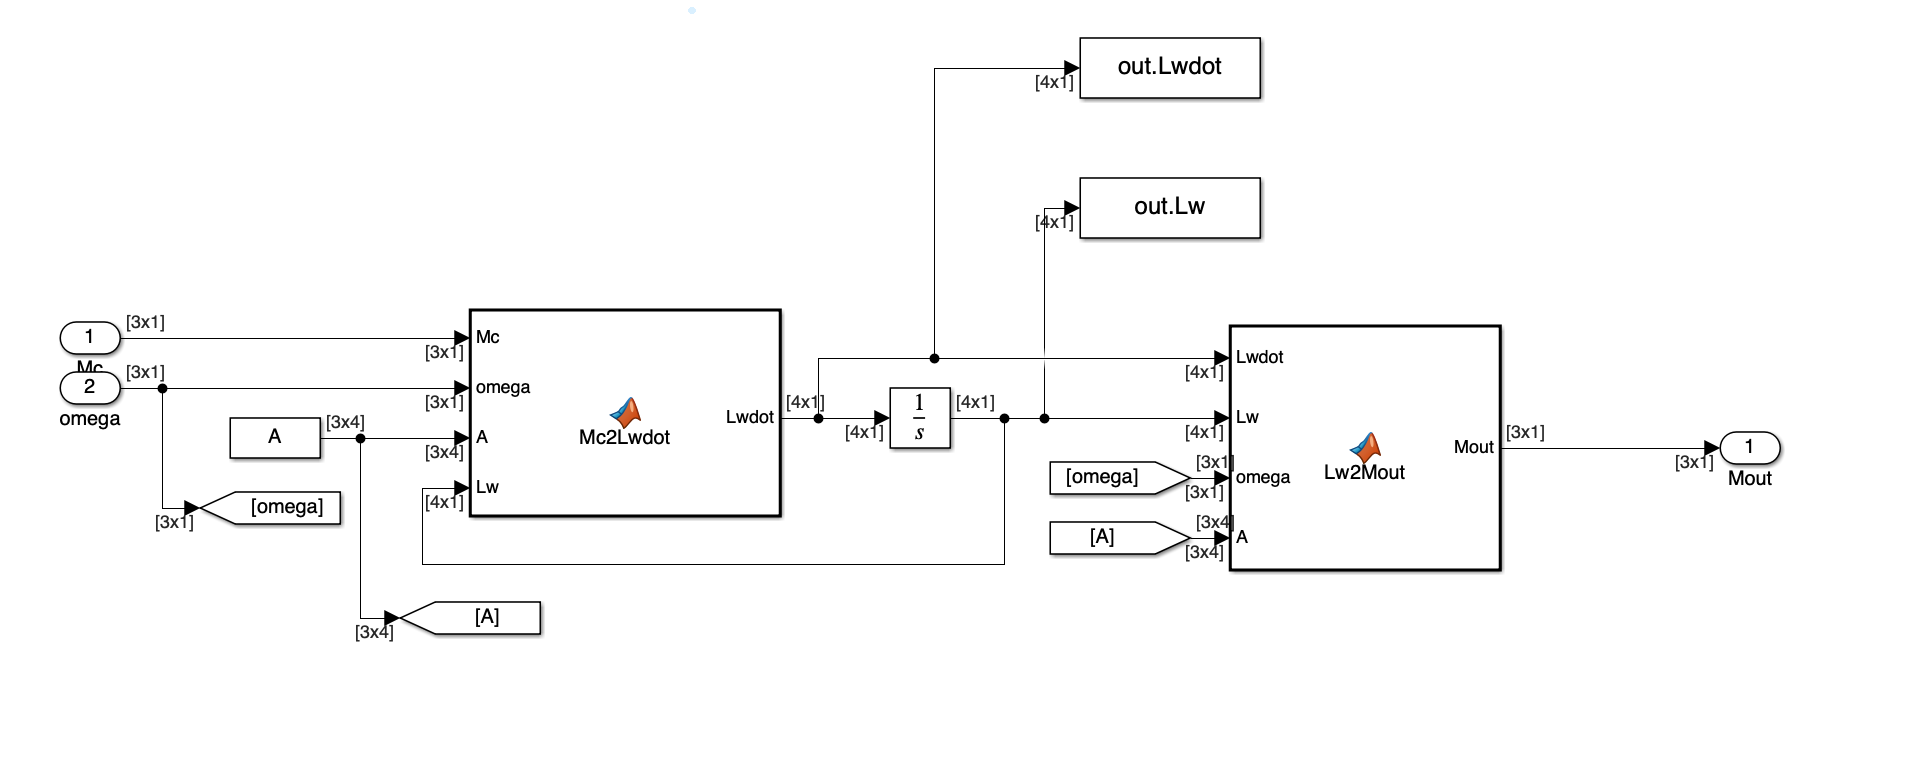
\includegraphics[width = 15cm]{Images/PS9/momentumWheelModel.png}
    \caption{Simulink Model for Momentum Wheel}
    \label{fig:simulink_mw}
\end{figure}

\begin{figure}[H]
    \centering
    \captionsetup{ justification = centering}
    \begin{lstlisting}
function Lwdot = Mc2Lwdot(Mc, omega, A, Lw)

Lwdot = pinv(A) * (- Mc - cross(omega, A * Lw));
    \end{lstlisting}
    \caption{Reaction Wheel Function}
    \label{fig:rwCode}
\end{figure}

For the magnetorquer, the following Euler equation was used to get output torque where $A$ = [0 0 1]$^T$.

\begin{equation}
    \Vec{M}_c = \Vec{m} \times \Vec{B} + \Vec{A} \Vec{\dot L}_w
\end{equation}

The same simulink model used to obtain the magnetic field for both the magnetic disturbances and magnetometer was used, and the new overall simulink model is shown below.

\begin{figure}[H]
    \centering
    \captionsetup{ justification = centering }
    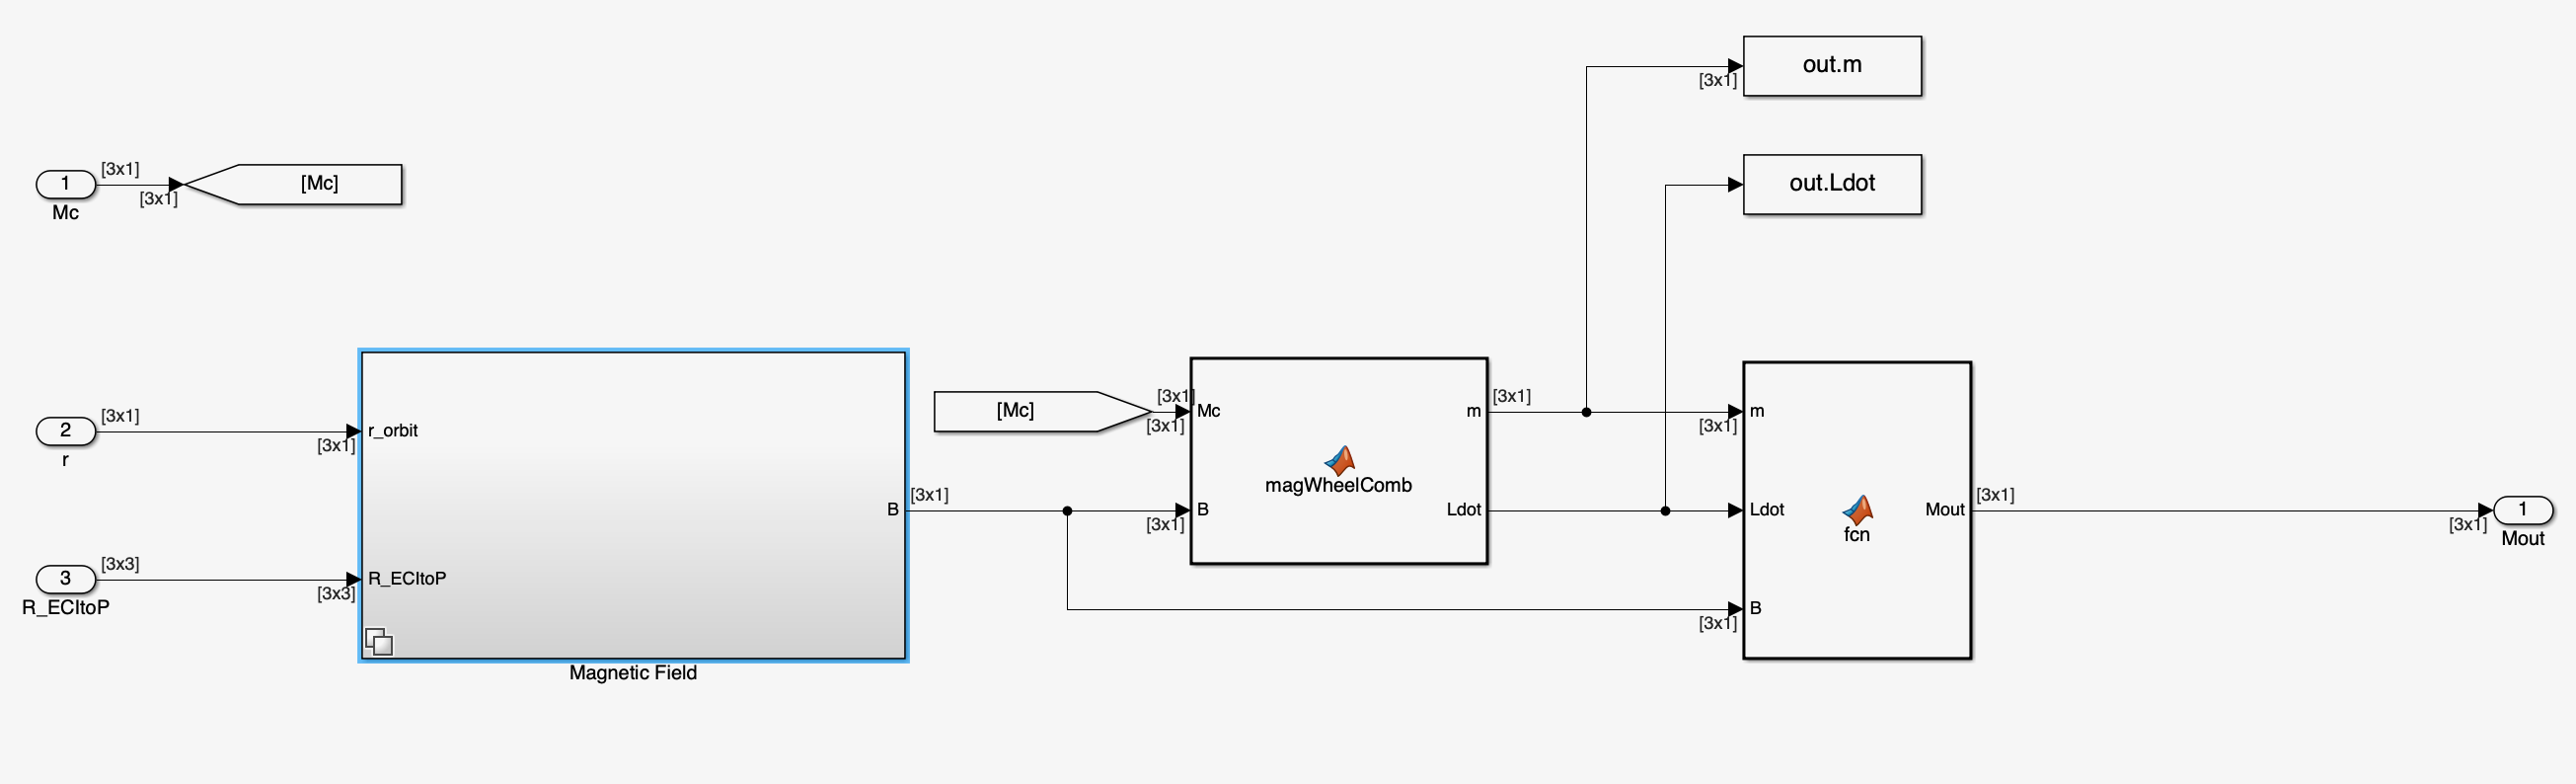
\includegraphics[width = 15cm]{Images/PS9/magnetorquerModel.png}
    \caption{Simulink Model for Magnetorquer}
    \label{fig:simulink_magnetorquer}
\end{figure}

\begin{figure}[H]
    \centering
    \captionsetup{ justification = centering}
    \begin{lstlisting}
function Mout = fcn(m, Ldot, B)

Mout = cross(m,B) + [0;0;1] * Ldot;
    \end{lstlisting}
    \caption{Magnetorquer Function}
    \label{fig:mtCode}
\end{figure}

The input and output of both of these actuators are shown below in Figures \ref{} and \ref{}.

\begin{figure}[H]
    \centering
    \captionsetup{ justification = centering }
    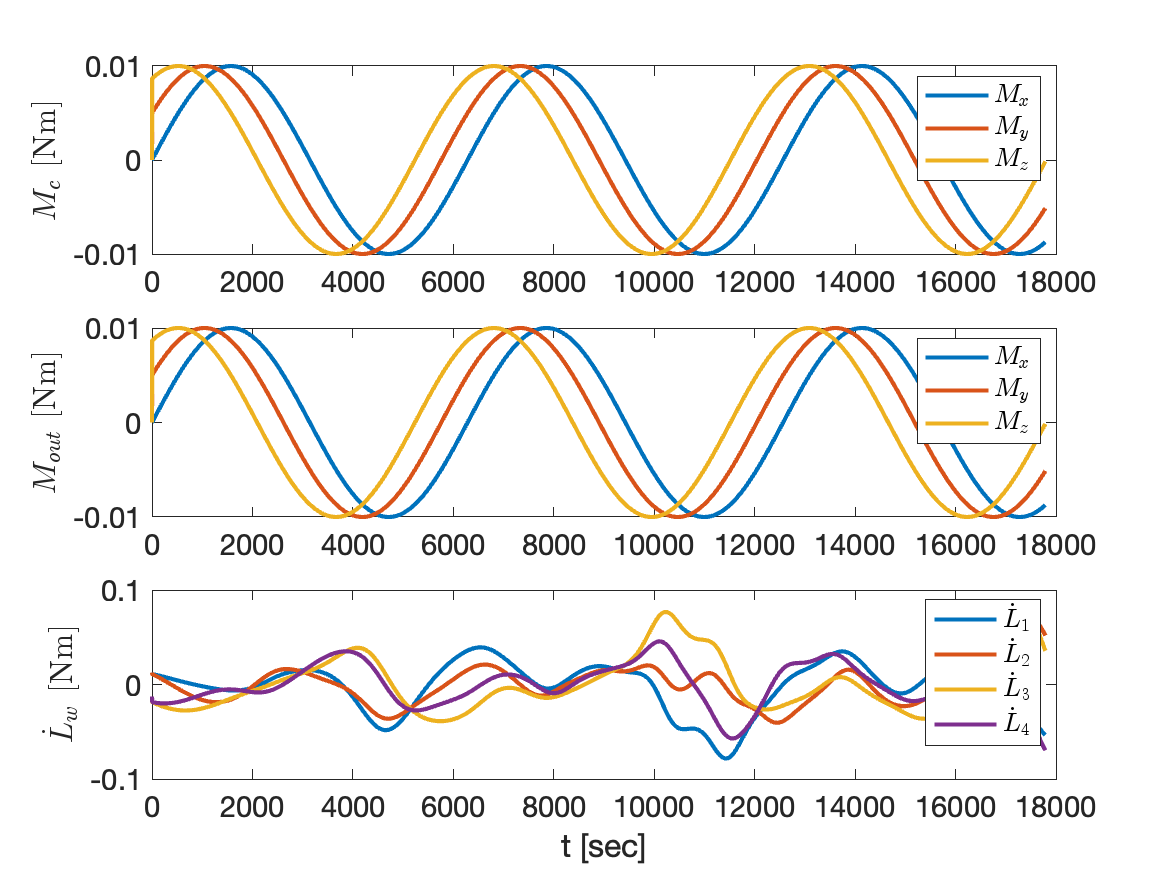
\includegraphics[width = 15cm]{Images/PS9/reaction_wheel_model_output.png}
    \caption{Output for Reaction Wheel}
    \label{fig:rwOutput}
\end{figure}

\begin{figure}[H]
    \centering
    \captionsetup{ justification = centering }
    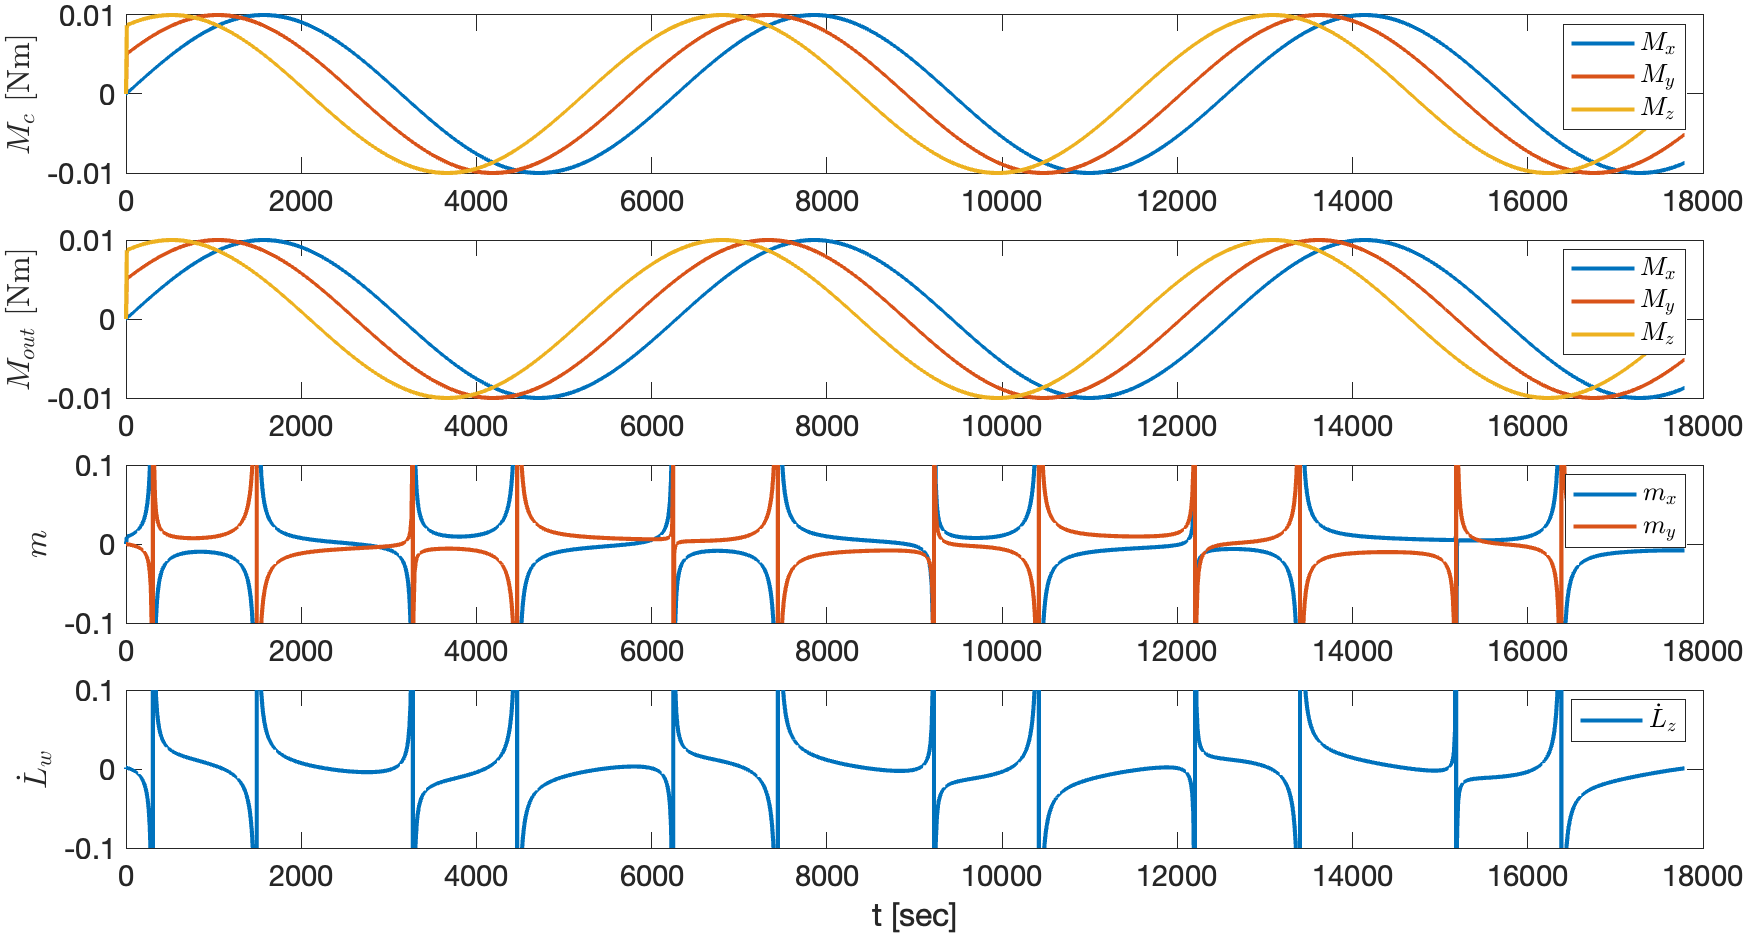
\includegraphics[width = 15cm]{Images/PS9/simple_magnetorquer_plus_wheel_model_output.png}
    \caption{Output for Reaction Wheel and Magnetorquer}
    \label{fig:mtOutput}
\end{figure}

\subsection{Problem 3 - Start designing and implementing a linear control law which provides the desired behavior of the dynamic system (damping and frequency) by a feedback done on the control tracking errors. Try using both a small angle approximation and a non-linear approach in defining the control tracking errors used in the control law. Hint: this task requires that you linearize the Euler equations and that you show how the gains of the linear control law are derived, also start applying the control law by assuming that the actuators are doing their job ideally (no actuation equations, no saturation or other limits). Selection of gains can be done through standard PD, pole placement or LQR approaches.}

A PD controller was used for this task. The nonlinear approach was done by taking the error produced from the sensor measurements, $R$, and producing the inverse skew matrix through the function shown in Figure \ref{fig:smallThetaCode}.

\begin{figure}[H]
    \centering
    \captionsetup{ justification = centering}
    \begin{lstlisting}
function alpha = inv_skw(R)

alpha = zeros([3 1]);

alpha(1) = (R(2,3) + (-R(3,2)))/2;
alpha(2) = (R(3,1) + (-R(3,1)))/2;
alpha(3) = (R(1,2) + (-R(2,1)))/2;
    \end{lstlisting}
    \caption{Small Angle Approximation Function}
    \label{fig:smallThetaCode}
\end{figure}

The small angle approximation was also attempted, but since the nonlinear approximation was functioning and the two approaches behaved the same in the relevant regime, it wasn't explored further. From here, $\alpha$ and the angular velocity errors from the gyroscope were fed into the following equation for the PD control law as $e_\theta$ and $e_\omega$.

\begin{equation}
    \Vec{I} \Vec{\dot \omega} = \Vec{\tau} - \Vec{\omega} \times (\Vec{I} \Vec{\omega})
\end{equation}

\begin{equation}
    - \dot \omega_{desired} = -K_p e_\theta - K_d e_\omega
\end{equation}

The simulink implementation of this is shown below.

\begin{figure}[H]
    \centering
    \captionsetup{ justification = centering }
    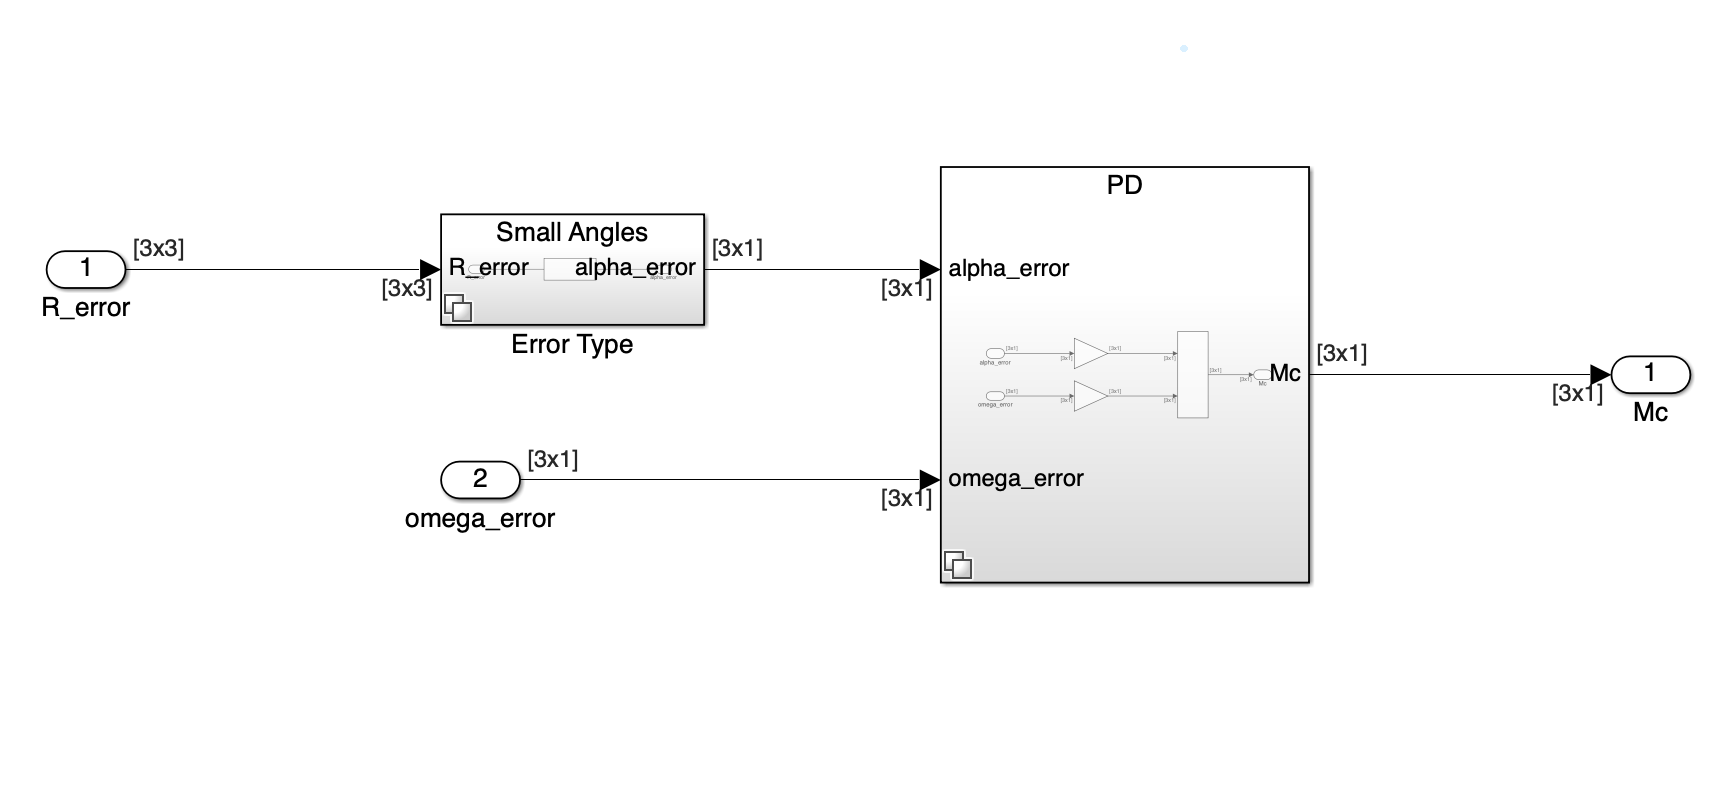
\includegraphics[width = 15cm]{Images/PS9/controllerModel.png}
    \caption{Simulink Model for Controller}
    \label{fig:controllerSimulink}
\end{figure}

\begin{figure}[H]
    \centering
    \captionsetup{ justification = centering }
    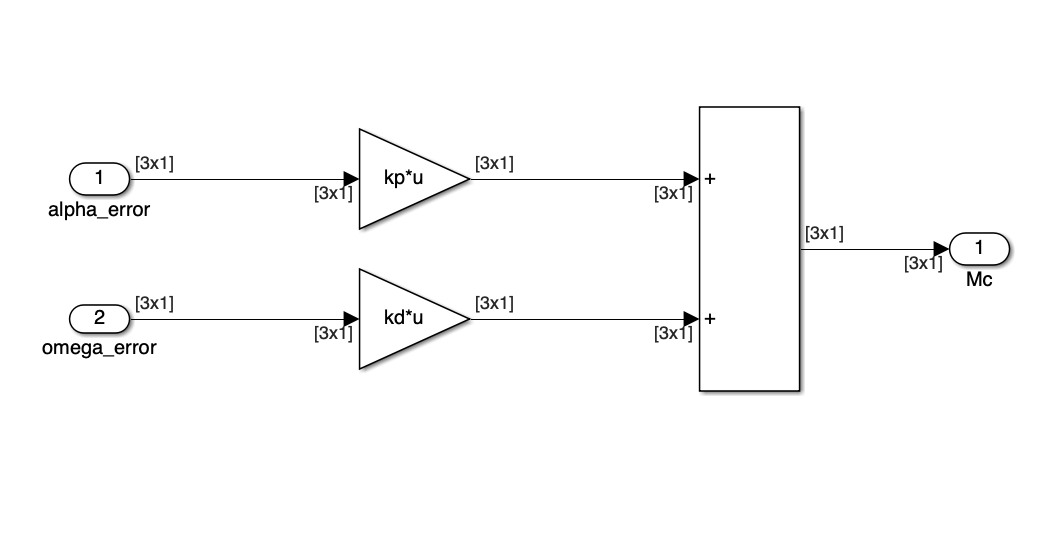
\includegraphics[width = 15cm]{Images/PS9/PDController.png}
    \caption{Simulink Model for PD Gains}
    \label{fig:PDsimulink}
\end{figure}

The design the $k_p$ and $k_d$ gains, the euler equations were linearized to follow the form shown below.

\begin{equation}
    I \Vec{\Ddot{\alpha}} + k_d  \Vec{\dot \alpha} + k_p \alpha = 0
\end{equation}

Additionally, the desired characteristic equation for the closed-loop transfer function is $s^2 + 2\zeta\omega_n s +\omega_n^2$ where $\zeta$ is the damping ratio and $\omega_n$ is the natural frequency. Because of this, $K_p = \omega_n^2 I_{axis}$ and $K_d = 2\zeta\omega_n I_{axis}$. From this, a damping ratio of $\sqrt{2}/2$ and a frequency of 50n were chosen to obtain $k_p$ and $k_d$.

It is also important to note that since there are currently bugs in our Kalman filter, the controller is currently getting fed ground truth to aboid residual errors.


\subsection{Problem 4 - Start plotting all the relevant quantities of your simulation, including attitude determination errors, attitude control errors, control actions (along all axes), etc. Hint: stress difference between what the ADCS believes, and what the spacecraft is actually doing. This affects estimation, control errors, and control actions.}

Due to bugs in our Kalman filter, the current attitutude determination error is getting plotted using the q-method as opposed to the MEKF.